\documentclass{article}
\usepackage{rotating}

\usepackage{tikz}
\usepackage{graphicx}
\usepackage{fontspec}
\usepackage{tocloft}
\usepackage{titletoc}
\usepackage{lipsum}  

\setmainfont{OpenSans-VariableFont_wdth,wght.ttf}[Path=assets/]

\begin{document}
%%%%%%%%%%    COVER    %%%%%%%%%%
\begin{titlepage}

\begin{flushright}

\vspace{7.5cm}

\Huge Team 1 EN.605.204.81 \\ ARM32 RSA Design Document

\vspace{0.5cm}

\Large Rohan Abraham, Tero Suontaka, Sullivan Prellwitz

\vspace{8cm}

\normalsize March 03, 2024

\end{flushright}

\end{titlepage}
\newpage
%%%%%%%%%%%%%%%%%%%%%%%%%%%%%%%%%
%%%%%%%%%%    LIST OF CONTENTS    %%%%%%%%%%
\tableofcontents
\newpage
%%%%%%%%%%%%%%%%%%%%%%%%%%%%%%%%%
%%%%%%%%%%    CONTENT    %%%%%%%%%%
\setmainfont{OpenSans-VariableFont_wdth,wght.ttf}[Path=assets/]
\section{Goals}
\setmainfont{OpenSans-VariableFont_wdth,wght.ttf}[Path=assets/]
Purpose: Encrypt and decrypt messages using a custom RSA implementation in ARM32 assembly.
Implement a modular design for all functions and create a library of assembly code that enables the generation of a public and private RSA keys using user specified values.
\newpage

\setmainfont{OpenSans-VariableFont_wdth,wght.ttf}[Path=assets/]
\section{Architecture}
\setmainfont{OpenSans-VariableFont_wdth,wght.ttf}[Path=assets/]
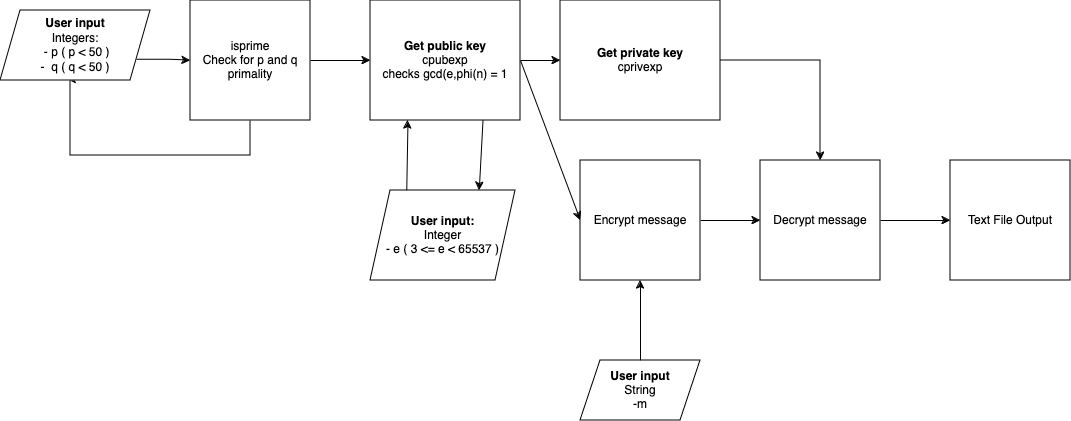
\includegraphics[scale=0.44]{assets/rsa-impl.drawio.png}
\section{Functions}
\setmainfont{OpenSans-VariableFont_wdth,wght.ttf}[Path=assets/]
    \subsection{gcd (Greatest Common Divisor)}
    Input: 2 integer values.
    \\
    Output: The greatest common divisor of the input integers.
    \\
    \subsection{pow}
    Input: 2 integer values, base \(b\) and an exponent \(e\).
    \\
    Output: \(b^e\)
    \\
    \subsection{mod (Modulo)}
    Input: 2 integers \(a\) and \(b\).
    \\
    Output: \(a \bmod b\)
    \\
    \subsection{tot (Totient Calculation)}
    Input: 2 prime numbers \(p\) and \(q\).
    \\
    Output: \(\phi (n) = (p-1)(q-1)\)
    \\
    \subsection{cpubexp (Calculation of public key exponent)}
    Input: 2 prime numbers \(p\) and \(q\), and an exponent \(e\) such that \(e\) is an integer
    and is not a factor of \(\phi (n) \) and \(1 < e < \phi (n)\).
    \\
    Output: Public key exponent.
    \\
     \subsection{cprivexp (Calculation of private key exponent)}
    Input: \(e\), \(\phi (n)\) an integer \(x\).
    and is not a factor of \(\phi (n) \) and \(1 < e < \phi (n)\)
    \\
    Output: Private key exponent.
    \\
    \subsection{encrypt}
    Input: An ASCII string plaintext to be encrypted and associated public key \(pubKey\).
    \\
    Output: ASCII string ciphertext
    \\
     \subsection{decrypt}
    Input: An ASCII string ciphertext and associated private key \(privKey\).
    \\
    Output: ASCII string plaintext
    \\
\newpage

\setmainfont{OpenSans-VariableFont_wdth,wght.ttf}[Path=assets/]
\section{Testability}
\setmainfont{OpenSans-VariableFont_wdth,wght.ttf}[Path=assets/]
    The individual components of the RSA implementation will be tested using a test script per function.
    These test scripts will cover normal, edge, and absurd cases in order to ensure proper functionality.
    The test scripts will be able to be run all at once using a control script.
    \\
    Test scripts will be help within a \verb|/tests| folder within the project repository and will take the form
    \begin{verbatim}
        {function_name}-tests.{file_extension}
    \end{verbatim}
\newpage

\setmainfont{OpenSans-VariableFont_wdth,wght.ttf}[Path=assets/]
\section{Timeline}
\setmainfont{OpenSans-VariableFont_wdth,wght.ttf}[Path=assets/]
    \subsection{March 11 - 15}
        \begin{itemize}
            \item First implementation meeting
            \item Initialize code repository
            \item mod function implementation finished, tests written
        \end{itemize}
    \subsection{March 25 - 29}
         \begin{itemize}
            \item Second implementation meeting
            \item gcd, pow, and tot implementation finished, tests written
            \item Plan next implementation steps
        \end{itemize}
    \subsection{April 8 - 20}
        \begin{itemize}
            \item Meet as needed
            \item RSA implementation finished (April 20), tests written
            \item Creation of testing control script
        \end{itemize}
    \subsection{April 21 - 27}
        \begin{itemize}
            \item Complete testing
            \item Squash bugs
            \item Prep repository and extra materials for submission
        \end{itemize}
    \subsection{April 28}
        \begin{itemize}
            \item Submit implementation
        \end{itemize}
\newpage

%%%%%%%%%%%%%%%%%%%%%%%%%%%%%%%%%
\end{document}

\begin{comment}

\end{comment}